\documentclass[12pt,a4paper,french]{article}
\usepackage[utf8]{inputenc}
\usepackage{graphicx}
\usepackage{color}
\usepackage{listings}

\usepackage{color}

\usepackage[francais]{babel}

\usepackage{amsmath}
\usepackage{graphicx}
\usepackage{amssymb}
\usepackage{float}

\usepackage{hyperref}

 \usepackage{enumitem}

\usepackage[sorting=none]{biblatex}
\addbibresource{ref.bib}

\definecolor{dkgreen}{rgb}{0,0.6,0}
\definecolor{gray}{rgb}{0.5,0.5,0.5}
\definecolor{mauve}{rgb}{0.58,0,0.82}

\newcommand\secspacing{1.5cm}
\newcommand\subsecspacing{1cm}

\usepackage{geometry}
\geometry{hmargin=2.5cm,vmargin=2.5cm}

\title{\LARGE{Projet PRAT : Rain Nowcasting} \\ [0.25cm]\large{Rapport bibliographique} \\ [2cm]}
\author{Lucas Beretti \\ [0.5cm]Encadrant : Dominique Béréziat \\ [2cm]}
\date{8 novembre 2021}

\begin{document}

\maketitle

\vspace{5cm}
\begin{center}
    \includegraphics[width=10cm]{images/Logo_Sorbonne_Université.png}
\end{center}

\newpage

\tableofcontents

\newpage

\section{Introduction}

Tout au long de son histoire, l'homme s'est intéressé au domaine de la prévision météorologique du fait de la forte dépendance de ses activités à celui-ci. Aujourd'hui encore, elle joue un rôle central dans de nombreux secteurs météo-sensibles comme l'agriculture, le transport, l'énergie, le tourisme ... Bien que les méthodes d'estimation de la météo se sont largement améliorées au cours des dernières décennies, la fiabilité de ces modèles est un sujet sur lequel les météorologues travaillent encore.

La prévision du taux de précipitation est une donnée cruciale pour l'ensemble des secteurs météo-sensibles. Ces prévisions sont effectuées par des modèles physiques intégrant divers phénomènes liés à la dynamique de l'atmosphère. Bien que ces méthodes apportent de bonnes prévisions de précipitation sur plusieurs jours, elles manquent encore de précision à très court terme, jusqu'à deux heures à l'avance. Cette problématique est plus communément appelée "Rain Nowcasting".

L'émergence des technologies d'apprentissage automatique, et plus précisément d'apprentissage profond, a amené certains chercheurs à s'intéresser à ce problème. 

Cet état de l'art a pour but de présenter un panel de méthodes élaborées au cours des dernières années sur des images radar. Ensuite, l'objectif sera d'implémenter et de comparer quelques méthodes sur des données radar de Météo-France. 

\vspace{\secspacing}

\section{Méthodes traditionnelles}

Cette partie a pour but de présenter quelques méthodes traditionnelles pour la prévision à court terme du taux de précipitation. De manière abusive, nous qualifierons de méthodes traditionnelles toutes les méthodes établies avant l'émergence de l'intérêt pour les techniques d'apprentissage profond appliquées à la résolution de cette problématique.

\vspace{\subsecspacing}

\subsection{Mise en correspondance de blocs d'images}

Les plus anciens types d'approches sont celles par mise en correspondance de blocs d'images. \newline

\textit{Tracking Radar Echoes by Correlation} (TREC) \cite{Rinehart:1978} est la première de ce type. Elle consiste à comparer des images de réflectivité des ondes radar d'une même zone acquises à quelques minutes d'intervalle. Chaque image va être découpée en blocs de même taille séparés par une distance donnée. Chaque bloc de la première image acquise va être comparé à l'ensemble des blocs de la seconde. Les coefficients de corrélation entre les motifs de réflectivité dans les blocs sont calculés pour toutes les paires de blocs possibles, et la paire avec le coefficient de corrélation le plus élevé est sélectionnée pour la détermination du vecteur de mouvement qui indique le mouvement du bloc d'origine pendant la période de temps $ \Delta{t} $.
Une fois le champ de mouvement calculé (c'est à dire que le vecteur de déplacement a été calculé pour l'ensemble des blocs), est alors obtenu un champ de mouvement de réflectivité qui va être utilisé pour estimer le déplacement des blocs, et donc les précipitations, par extrapolation. Ces précipitations sont adaptées à chaque nouvelle acquisition faite par la mise à jour du champ de mouvement de réflectivité. 

Cette méthode est très sensible à de nombreux paramètres comme la taille des blocs, la distance séparant le centre de deux blocs, la taille de la grille des données radar, l'intervalle de temps entre deux acquisitions. Elle est efficace pour décrire le mouvement de cellules pluvieuses mais ne permet pas de prendre en compte le mouvement global à plus grande échelle de la structure orageuse. Enfin, le vecteur de mouvement se veut parfois incohérent et bruité. La principale cause est le phénomène de fouillis de sol, lorsque d'autres éléments sont détectés, tels que des oiseaux, des insectes, des objets près du sol et de la poussière. Ces échos de fouillis génèrent des trous dans le champ de mouvement de réflectivité \cite{1995JApMe..34.1286L}. \newline

Des solutions à ces différents problèmes ont été développées. \textit{Continuity of Tracking Radar Echoes by Correlation} (COTREC) vise à corriger le bruit causé par le phénomène de fouillis de sol \cite{1995JApMe..34.1286L}. Enfin, la méthode \textit{Multi-scale Tracking Radar Echoes by Correlation} (MTREC) intègre de manière plus globale le mouvement de la structure orageuse. En effet, elle consiste en l'application de la méthode TREC avec des blocs de tailles différentes pour décrire les phénomènes locaux et plus globaux \cite{120026}. \newline


\vspace{\subsecspacing}

\subsection{Mise en correspondance de cellules de précipitations}

Les méthodes de mise en correspondance de cellules de précipitations sont assez proches, dans leur fonctionnement, de celles de correspondance de blocs d'images. Cependant, au lieu de segmenter l'ensemble de l'image en blocs, un premier algorithme va identifier les cellules et leurs caractéristiques sur l'image. Ensuite, différentes méthodes existent pour la mise en correspondance des cellules identifiées entre deux images. \newline

L'approche \textit{CELLTRACK} va prendre en compte un critère de similarité de forme entre le coeur d'une cellule (la zone de réflectivité maximale au sein d'une cellule pluvieuse) d'une première image et les coeurs des cellules de la seconde. A cela s'ajoute la notion de la distance euclidienne entre les coeurs des cellules. L'algorithme essaye dans un premier temps d'apparier les clusters de cellules proches car ce sont les plus susceptibles d'être sujet à des séparations et fusions des noyaux de réflectivité. Comme pour les approches par blocs, les prévisions sont effectuées par extrapolation du vecteur de mouvement estimé entre deux acquisitions radar \cite{celltrack}. 

\vspace{\subsecspacing}

\subsection{Méthodes s'appuyant sur le flot optique}

Le majeur inconvénient des méthodes précédentes est que le calcul du vecteur de vitesse du déplacement se limite aux blocs ou aux cellules de précipitations identifiées. Ainsi, hormis MTREC qui s'applique à plusieurs échelles, elles semblent plus adaptées à décrire le mouvement de blocs ou de cellules de précipitations individuelles plutôt que le mouvement global. \newline

Les approches par flot optique apportent des solutions à ces problématiques. Elles calculent des vecteurs de déplacement en tout pixel de l'image et utilisent des images à plusieurs échelles pour prendre en compte le comportement météorologique à large et plus fine échelle. \cite{atmos8030048} \newline

Ces modèles partent de l'hypothèse de la conservation de la réflectivité au fil du temps le long des trajectoires. Cette hypothèse se traduit par une relation à laquelle il n'est pas possible d'obtenir une unique solution de par son nombre d'inconnues. Il est alors nécessaire d'introduire des contraintes supplémentaires sous la forme d'un problème de minimisation d'une fonction de coût, ayant pour but d'assurer la continuité et la régularité du gradient. C'est ce qui est fait dans la méthode \textit{Multi-Scale Optical-Flow by Variational Analysis} (MOVA) \cite{atmos8030048}. Des fenêtres de différentes tailles sont appliquées pour le calcul du vecteur de déplacement des pixels. L'algorithme est en cascade : une première estimation du champ vectoriel est calculée pour la fenêtre de taille la plus grande correspondant au comportement météorologique dans sa globalité. Ce résultat va être affiné de manière itérative par réduction de la taille de la fenêtre et donc, la prise en compte de phénomènes plus locaux. 

La méthode \textit{Real-Time Optical Flow by Variational Methods for Echoes of Radar} (ROVER) (aussi dans \cite{atmos8030048}) est similaire à MOVA mais ajoute une étape de pré-traitement pour lisser les données et augmente la vitesse des calculs en utilisant une fonction de coût différente.

Les champs de mouvement estimés par ces méthodes sont utilisés pour calculer les prévisions du taux de précipitations par extrapolation. 
\newline

Par la prise en compte des phénomènes physiques de l'atmosphère, les approches par flot optique semblent plus adaptées pour décrire le mouvement des cellules nuageuses au cours du temps que les méthodes par association de blocs ou de cellules qui reposent sur une association entre deux images. C'est d'ailleurs la conclusion tirée de l'article \cite{atmos8030048} : ROVER et MOVA obtiennent de meilleures prévisions que TREC.  

\vspace{\secspacing}

\section{Méthodes par apprentissage profond}

Nous avons vu, sans trop entrer dans les détails, différentes approches au problème "Rain Nowcasting". L'émergence des méthodes d'intelligence artificielle ont poussé des chercheurs à s'intéresser à l'application de celles-ci.

Différentes démarches par apprentissage profond ont été étudiées durant les dernières années : des réseaux de neurones récurrents, U-Net et réseaux antagonistes génératifs (GAN). 

\vspace{\subsecspacing}

\subsection{Approches récurrentes}

\vspace{\subsecspacing}

\subsubsection{ConvLSTM}

L'observatoire de Hong Kong a développé le premier modèle d'apprentissage profond pour répondre à ce problème. Ses résultats sont comparés à la méthode ROVER. Cette dernière, bien qu'efficace possède de nombreux paramètres qui sont difficiles à déterminer pour donner de bonnes performances de prédiction. Par conséquent, des réseaux de neurones peuvent être capable d'apprendre à calculer le flot optique, comme le fait l'algorithme ROVER, sans avoir à définir différents paramètres au préalable. 
\newline

La motivation qui a poussé les auteurs de ce papier à s'intéresser à un réseau récurrent convolutif provient de la recherche de travaux sur une problématique similaire. En effet, ce type d'architecture a été retenu pour la prédiction de la prochaine image dans une vidéo \cite{Ranzato2014Video}. \newline

Dans \cite{shi2015convolutional}, les auteurs se sont basés sur l'architecture récurrente \textit{Long Short Term Memory} (LSTM) en ajoutant des opérations de convolutions pour garder l'information spatiale présente au sein des images. Ces couches se nomment ConvLSTM. 
Plusieurs couches ConvLSTM sont utilisées pour créer une architecture encodeur décodeur. Ainsi, les premières couches de l'encodeur vont permettre d'identifier des phénomènes plutôt locaux alors que les plus profondes vont détecter des mouvements plus globaux pour avoir une compréhension plus fine du phénomène météorologique que par une analyse à une seule échelle. Cela rejoint les approches par flot optique qui traitaient les images à plusieurs échelles suite aux limites des méthodes initiales comme TREC qui était restreint par la taille des blocs. L'information va ensuite être décodé pour réaliser la prédiction. \newline

Le dataset choisi pour cette étude sont des données de réflectivité issues des radars météorologiques de Hong Kong. C'est donc un problème de régression pour l'estimation de la réflectivité (à noter qu'une relation relie la réflectivité au taux de précipitation). Ces données sont acquises toutes les 6 minutes et les séquences utilisées comportent 20 images (5 pour l'entraînement et 15 pour les prédictions). Les 97 jours les plus pluvieux ont été sélectionnés pour l'entraînement du modèle. 

Différentes métriques sont utilisées pour évaluer les performances du modèle dont certaines se basant sur des valeurs binaires. Par conséquent, un seuil à un taux de précipitation de 0.5mm/h a été utilisé (valeur limite à laquelle il est considéré qu'il pleut).

Pour l'ensemble des métriques évoquées, les résultats obtenus par le réseau ConvLSTM sont meilleurs que l'approche par flot optique ROVER et que le réseau LSTM non convolutif. De même, la dégradation de la précision des prédictions diminue plus lentement pour le réseau récurrent convolutif. 
\newline

Certaines remarques sont à tirer de cet article : 
\begin{enumerate}
    \item l'approche LSTM semble être adaptée par sa capacité à abandonner de l'information. Cependant, les méthodes par flot optique se basaient sur l'information des deux ou trois dernières images pour la prédiction des suivantes. Le réseau est alors peut-être trop complexe pour la tâche à réaliser.
    \item la manière d'évaluer les performances du réseau ne permet pas d'estimer si ce dernier obtient de bonnes prédictions à taux de précipitation plus élevé. Or, ceci constituerait une information importante pour de nombreux secteurs d'activité météo-sensible.
    \item la construction du dataset avec les 97 jours les plus pluvieux est discutable malgré la justification dans l'article que l'objectif du réseau est de prédire la pluie et que tous les jours ne sont pas pluvieux. Ce choix va biaiser le modèle lors de son utilisation opérationnelle. 
\end{enumerate}

\vspace{\subsecspacing}

\subsubsection{TrajGRU}

Les chercheurs ayant travaillé sur le modèle ConvLSTM, évoqué dans la partie précédente, ont planché sur une nouvelle approche après avoir identifié deux défauts majeurs : 

\begin{enumerate}
    \item la propriété d'invariance par localisation des filtres convolutifs utilisés qui ne permet pas de décrire fidèlement les phénomènes météorologiques. Les hyperparamètres des filtres convolutifs sont fixes (notamment la taille du noyau, le paramètre de dilatation). Par exemple, dans le cadre d'une rotation ou d'un changement d'échelle d'une cellule pluvieuse, la convolution aurait des difficultés pour rendre compte du phénomène comparé à une méthode basée sur le flot optique.
    \item le dataset utilisé pour l'entraînement et la manière d'évaluer le modèle. En effet, ils reconnaissent que choisir les 97 jours les plus pluvieux comme données d'entraînement du modèle créé un biais. De plus, utiliser un seuil à 0.5 mm/h de pluie pour évaluer les performances du modèle n'est pas efficace pour rendre compte de son bon fonctionnement, notamment à haut taux de précipitation. 
\end{enumerate}

Partis de ce premier constat, ils ont proposé le modèle TrajGRU qui est convolutif et récurrent. Ce modèle utilise l'adaptation convolutive de la cellule \textit{Gated Recurrent Unit} (GRU). 

La particularité du modèle TrajGRU est d'apprendre les connections récurrentes de manière dynamique. 

\begin{figure}[H]
\centering
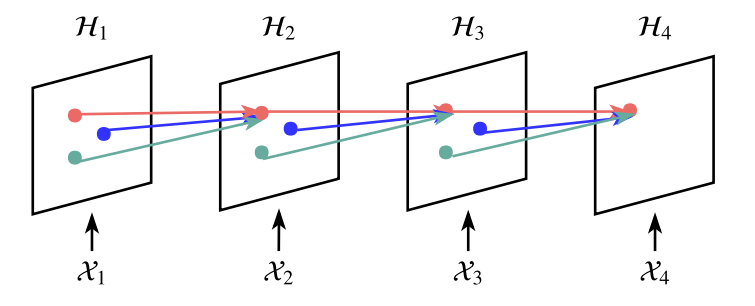
\includegraphics[scale=0.5]{images/liaison_tradi_CNN.png}
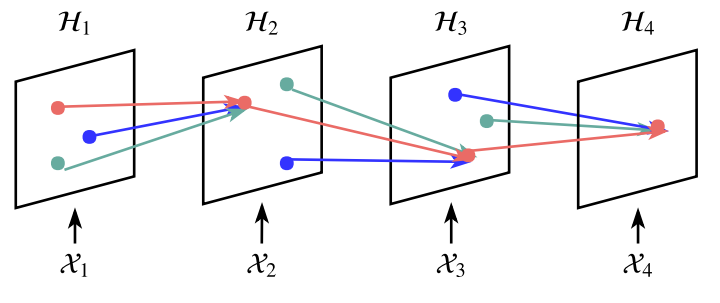
\includegraphics[scale=0.5]{images/liaison_traj_gru.png}
\caption{Comparaison de la structure des connections entre un réseau convolutif récurrent classique (en haut) et le modèle TrajGRU (en bas). Images issues de \cite{shi2017deep}.} 
\end{figure}

Ainsi, pour apprendre de manière automatique les connections récurrentes, un réseau de neurones convolutif $ \gamma $ à une couche cachée a été utilisé. C'est donc un réseau très simple avec peu de paramètres. Il se base sur l'entrée à l'instant $ t $ $ X_{t} $ et l'état en mémoire à l'instant $ t-1 $ $ H_{t-1} $. Les vecteurs de déplacement horizontaux et verticaux à l'instant $ t $ sont alors estimés comme : $ U_{t}, V_{t} = \gamma(X_{t}, H_{t-1}) $. \newline

Le réseau utilisé dans ce papier est une structure encodeur-décodeur avec des cellules TrajGRU, du sous-échantillonage dans la partie encodeur et du sur-échantillonage dans le décodeur pour détecter des phénomènes à diverses échelles. \newline

Sur la base du deuxième constat effectué, les auteurs ont changé la manière de créer le dataset. En effet, ils ont sélectionné l'ensemble des jours pluvieux (993 jours, ce qui est significativement plus que les 97 jours utilisés dans \cite{shi2015convolutional}). En effet, ils souhaitent utiliser le modèle de prévision du taux de précipitation seulement si un premier modèle a indiqué la veille s'il allait pleuvoir ou non. 

Ils ont aussi pris en compte les limites de l'évaluation du modèle dans \cite{shi2015convolutional}. Premièrement, ils ont utilisé une erreur quadratique moyenne pondéré par un poids face au problème du déséquilibre du jeu de données vis-à-vis des différents niveaux de précipitations. En effet, la plupart des pixels du jeu de données correspondent à un taux de précipitation compris entre 0 et 0.5 mm/h indiquant pas de pluie ou très peu alors que seulement 1.56\% ont un taux supérieur à 10 mm/h. De plus, plusieurs seuils de taux de précipitation ont été utilisés pour mieux rendre compte des performances du modèle lors l'évaluation avec des indicateurs binaires. Dans cet article, le problème est toujours de régression et les données sont des données de réflectivité. L'estimation du taux de précipitation se base sur la relation $ Z - R $.

Enfin, il a été testé deux configurations différentes : un modèle entraîné normalement (qui, à partir de 5 images prédit les 20 suivantes) et un modèle entraîné auquel, lors de la phase de prédiction opérationnelle, on applique un réajustement des poids au fur et à mesure que le modèle reçoit des séquences de 5 images (on qualifie de \textit{online fine-tuning}). Cette deuxième méthode semble particulièrement adaptée opérationnellement car le modèle continue d'apprendre au fil du temps. \newline

Les performances du modèle TrajGRU ont été comparées à d'autres modèles : l'approche ROVER basée sur le flot optique, des CNN classiques 2D et 3D (structure d'un Encodeur-Decodeur convolutionnel sans \textit{skip-connections}), un modèle ConvGRU (même architecture que le TrajGRU sans les connections récurrentes dynamiques) et un modèle ConvGRU entrainé sans la fonction de perte pondérée pour équilibrer le jeu de données comme dans \cite{shi2015convolutional}. Le modèle TrajGRU performait mieux que l'ensemble des autres modèles selon l'ensemble des indicateurs et pour tous les taux de précipitations considérées. De plus, l'ensemble des modèles où le \textit{online fine-tuning} a été appliqué a obtenu de meilleurs résultats par rapport aux mêmes modèles sans cet ajustement. Il est intéressant de noter que le modèle ConvGRU entraîné sans ajustement de la fonction de perte pondérée (similairement à \cite{shi2015convolutional} performait moins bien que l'approche par flot optique pour un taux de précipitation moyen ou élevé. \newline

On peut émettre quelques remarques sur cet article :
\begin{enumerate}
    \item cette article ne justifie pas le choix de l'utilisation d'un GRU convolutif vis-à-vis du modèle LSTM. On peut penser que c'est parce que le modèle GRU est légèrement plus simple que le modèle LSTM et qu'une telle complexité n'était pas nécessaire pour décrire le mouvement des cellules pluvieuses. Cette critique rejoint celle effectuée dans la partie précédente.
    \item il n'est pas mentionné comment est entraîné le modèle $ \gamma $ qui est responsable de déterminer les connections récurrentes.
    \item l'utilisation de jours seulement pluvieux pour la création du jeu de données est discutable. Certaines journées peuvent être pluvieuses avec un très faible taux de précipitations. Cependant, cela prend sens dans le cas de l'\textit{online fine-tuning}, puisque trop de jours sans pluie pourraient faire dévier les performances du modèle, le rendant moins efficace à la prévision des précipitations. 
\end{enumerate}

\vspace{\subsecspacing}

\subsection{Approches U-Net}

Dans cette partie, nous allons nous intéresser aux réseaux U-Net. Plusieurs travaux se sont intéressés à l'utilisation de ce type de réseau pour répondre à la problématique de prévision de la précipitation. \newline

Un premier article est particulièrement intéressant, puisqu'il construit un modèle U-Net et compare ses résultats à l'approche TrajGRU évoquée dans la partie précédente. L'entrée du réseau U-Net comporte 5 images radar de réflectivité consécutives. C'est un problème de régression.

Il montre que les résultats obtenus entre les deux modèles sont semblables : U-Net performe légèrement mieux à haut taux de précipitation que TrajGRU et inversement.  

Cet article tire donc la conclusion que le U-Net utilisé, un modèle assez simple de part sa construction avec 4 couches convolutives dans l'encodeur et le décodeur, obtient des résultats comparables à un modèle beaucoup plus complexe qui est le TrajGRU, particulièrement adapté à l'apprentissage de séries temporelles. \cite{9508500}

Par conséquent, cela pose la question de l'intérêt de l'utilisation de modèle récurrent, ces derniers ne sont peut être pas si adaptés pour décrire ce phénomène météorologique. \newline

Il faut tout de même noter que l'étude développée dans \cite{9508500} ne s'intéressait qu'aux précipitations dans les 30 prochaines minutes (et donc à la prédiction de 5 images). Nous n'avons donc pas idée des performances à plus long terme. \newline

L'article \cite{bouget:hal-03112093} se propose d'ajouter les données de vent en entrée du réseau de neurones en plus des données de précipitations. Contrairement à l'ensemble des articles évoqués précédemment qui se basent sur des images radar de réflectivité, le cumul des précipitations sur 5 minutes est utilisé. La sortie du modèle correspond aux cartes de prédictions des cumuls de précipitation. 

Le problème est de classification. 3 seuils sont utlisés pour caractériser l'intensité de la pluie : 0.1 mm/h, 1 mm/h, 2.5 mm/h. 

Les résultats montrent que le modèle intégrant les données de vent apportent de meilleurs résultats que le même modèle avec seulement les images de pluie. Par conséquent, on peut déduire de cet article que la prise en compte de données de vent apportent une réelle plus-value pour la qualité des prédictions. 

\vspace{\subsecspacing}

\subsection{Approche par réseau de neurones génératif}

L'utilisation d'un réseau GAN développé dans \cite{Ravuri2021SkilfulPN} repose principalement sur une idée : bien que les modèles d'apprentissage profond prédisent avec précision les précipitations de faible intensité, leur utilité opérationnelle est encore limitée car ils manquent de contraintes. Par conséquent, ils ont tendance à produire des prévisions floues à des délais plus longs, entraînant de mauvaises performances pour des évènements de prévision de pluie à moyenne ou haute intensité puisque ces derniers sont les plus rares. Ainsi, l'utilisation de réseau de neurones génératifs va ajouter, de par l'utilisation de discriminateur, des contraintes supplémentaires forçant le modèle à produire des images de prévisions plus ressemblantes de la réalité et donc plus fiables à long terme. \newline

Le réseau retenu est constitué de deux discriminateurs et d'un générateur. Un discriminateur spatial est un réseau convolutif qui se charge de distinguer, de manière individuelle, des observations radar de celles qui sont générées ce qui impose la cohérence spatiale et limite la production de prévisions dont les contours sont flous. Un discriminateur temporel, qui un réseau convolutif 3D, tente de discerner les séquences observées des séquences générées, imposant une cohérence temporelle et pénalisant les prédictions sautillantes (ayant une grande variation temporelle d'une image à l'autre). Le modèle générateur a la forme d'un encodeur décodeur, comme l'ensemble des autres modèles utilisés. Il utilise des cellules récurrentes ConvGRU. Le problème est de régression. \newline

Les performances du réseau GAN sont comparées notamment à un réseau U-Net. A faible taux de précipitation, le réseau U-Net obtient de légers meilleurs résultats alors que le réseau GAN semble plus adapté pour des taux de précipitations plus élevés. Enfin, sur l'observation qualitative des résultats de manière visuelle, les contours des zones de précipitations sont plus fidèles à ce que l'on peut observer dans la réalité. En effet, le U-Net a tendance à produire des prédictions floues avec le temps. Par exemple, pour des prévisions à 90 minutes, la résolution des images produites est inférieure à 1 $ km^2 $ alors que celles produites par le U-Net ont une résolution de 32 $ km^2 $. Il est important d'avoir des images de bonnes résolutions notamment dans le cadre de précipitations très intenses qui sont souvent localisées. \newline

\vspace{\secspacing}

\section{Réalisation du projet}

\vspace{\subsecspacing}

\subsection{Données utilisées}

Pour ce projet, nous allons utiliser des données radars issues de MétéoNet, projet de Météo France. Elles recensent la pluie cumulative tombée sur une période de 5 minutes et ont été acquises par des radars Doppler entre 2016 et 2018. La zone d'étude choisie est la région Brestoise, étant donné que la qualité des données fournies par MétéoNet, c'est à dire leur fiabilité, est de 80\%, représentant un bon score vis-à-vis du reste de la France. Les images de pluie sont de tailles $ 128 \times 128 $  pixels soit une région de $ 100 km \times 150 km $. \newline

De plus, nous pourrons être amenés à ajouter des données de vent issu du modèle de prévision météorologique de Météo-France. Il donne, chaque jour, les prévisions des données de vent selon les composantes $ U $ (d'ouest en est) et $ V $ (sud vers le nord) avec une résolution spatiale d'1 $ km $. \cite{bouget:hal-03112093}

\vspace{\subsecspacing}

\subsection{Objectifs du projet}

Au cours de ce projet, je pourrais être amené à :
\begin{itemize}[label=--]
    \item comparer des approches de l'état de l'art au U-Net en \cite{bouget:hal-03112093}.
    \item étudier l'effet de l'ajout de données de vent sur l'amélioration des prédictions. 
    \item étudier d'autres approches avec un réseau générateur inspiré de l'architecture d'autres articles comme le U-Net par exemple.
\end{itemize}

\vspace{\subsecspacing}

\subsection{Calendrier prévisionnel}

\begin{itemize}[label=--]
    \item 26/10 : proposition de plan et papiers à citer.
    \item 08/11 : rapport bibliographique sur l'état de l'art.
    \item 08/11 - fin novembre : prise en main les données et implémentation de la chaîne d'entraînement et d'évaluation des réseaux de neurones. Premiers résultats sur un réseau convolutif simple.
    \item 01/12 - 17/12 (vacances de Noël) : implémentation d'un réseau intéressant de l'état de l'art (TrajGRU ou GAN).
    \item 17/12 - 15/01 : études de méthodes pour l'amélioration des solutions (ajout données de vent, autres réseaux générateurs si l'approche GAN est choisie, autres pistes à réflechir ...). 
    \item 15/01 - 07/12 : Rédaction du rapport et préparation pour la présentation orale. 
    \item 07/02 : Présentation orale du projet.
    
\end{itemize}

\newpage

\nocite{zebiri:tel-03127158}
\printbibliography[title=Références]

\end{document}
